\documentclass[../Article_Sensitivity_Analsysis.tex]{subfiles}
\graphicspath{{\subfix{../Figures/}}}
\begin{document}
	
	\begin{comment}
		
	\label{CH: Results}
	
	To identify the global solution of Equations \ref{EQ:Formulation_1}, the optimization problem is solved multiple times, each starting from a random initial solution. Figure \ref{fig:scatter_T} compares the initial and final values of the cost function across multiple optimization runs. The shaded area spans from the smallest to the third smallest final values of the objective function. The black curves on the left and below the scatter plot represent the distributions of the initial and final cost function values, respectively. From Figure \ref{fig:scatter_T}, it can be observed that multiple local solutions exist for Case 1. The solution with the lowest cost function value is considered the global solution.
	
	\begin{figure}[h!]
		\centering
		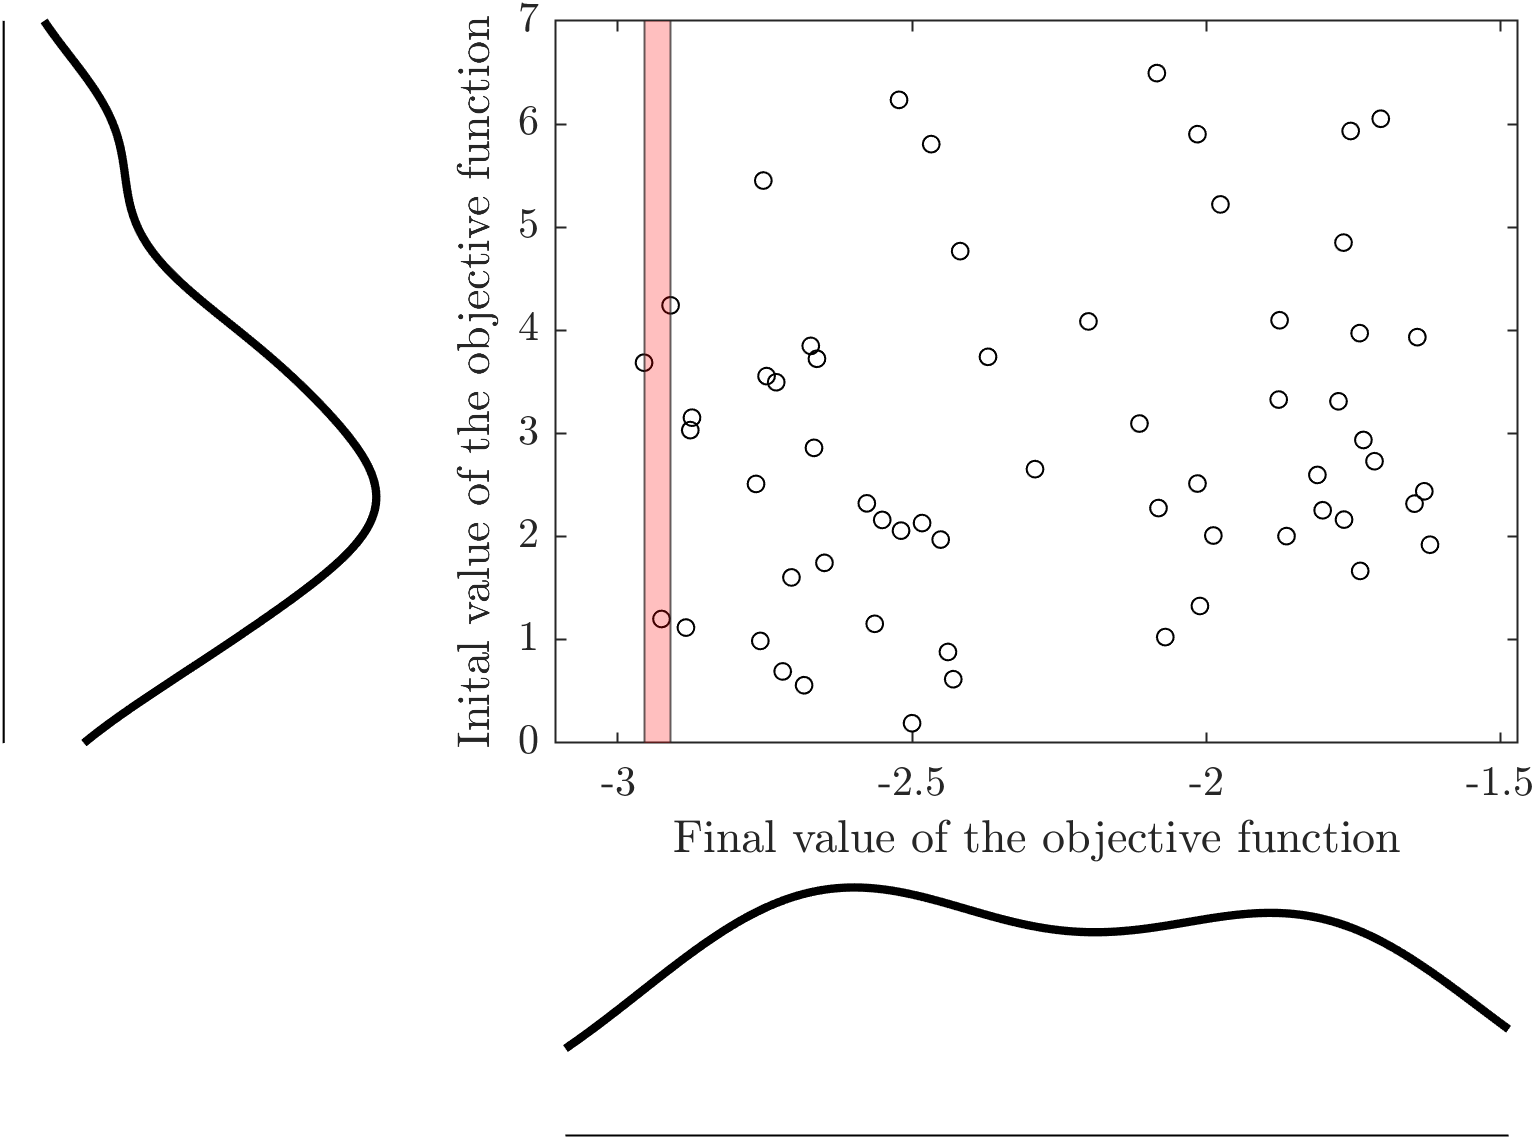
\includegraphics[width=\columnwidth]{Figures/Results/scatter_T.png}	
		\caption{Initial vs final values of the cost function}
		\label{fig:scatter_T}
	\end{figure}
	
	The optimal profiles of inlet temperature and mass flow rate are presented in Figure \ref{fig:profile_T}. One of the independent parameters in the analysed correlation is the mass flow rate, which is directly modified several times during the experiment. The second independent parameter is the Reynolds number, which can be affected by changes in the thermodynamic properties of the fluid. The thermal properties of CO$_2$ between $30^\circ$C and $40^\circ$C, assuming a constant pressure of 150 bar, vary only slightly. For instance, the dynamic viscosity changes from 67 to $80 \times 10^{-6}$ Pa$\cdot$s. The obtained profile of the inlet temperature shows minimal variation, suggesting a limited influence of inlet temperature on the extraction yield. Given the narrow operational window for inlet temperature at constant pressure, the mass flow rate becomes the primary variable to control.
	
	\begin{figure}[h!]
		\centering
		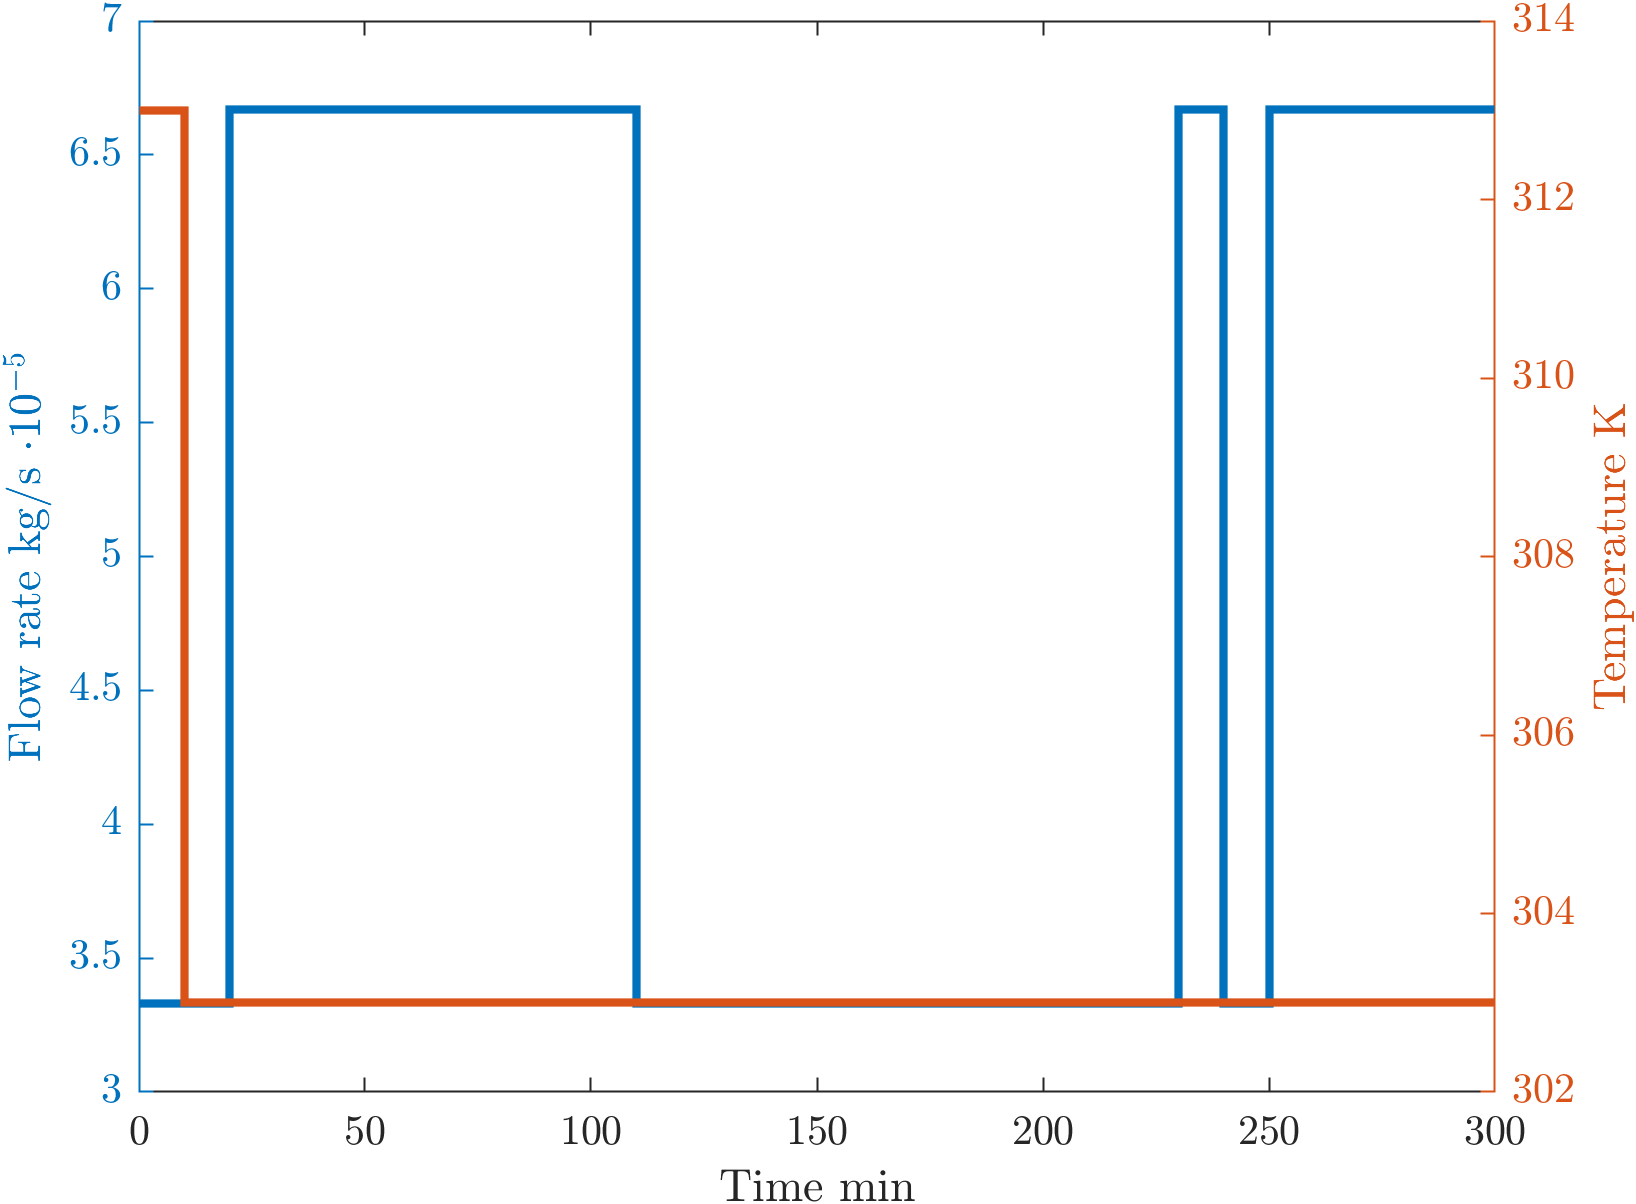
\includegraphics[width=\columnwidth]{Figures/Results/Profile_T_1.png}	
		\caption{Optimal temperature and mass flow rate profiles}
		\label{fig:profile_T}
	\end{figure}
	
	Similar to Case 1, Case 2 is solved multiple times starting from random initial solutions to identify the global solution. Figure \ref{fig:scatter_P} summarizes the changes in the objective function values across all optimization runs. It is evident that both the initial and final values of the cost function are significantly lower than any values obtained in Case 1. In Case 2, the wider operating range leads to more significant changes in the physical properties of CO$_2$ compared to Case 1. For example, the kinematic viscosity of CO$_2$ ranges from $48 \cdot 10^{-6}$ (at $40^\circ$C and 100 bar) to $90 \cdot 10^{-6}$ Pa$\cdot$s (at $30^\circ$C and 200 bar). The greater variability in pressure induces a more complex system response, including temperature variations, resulting in lower values of the objective function compared to Case 1.
	
	\begin{figure}[h!]
		\centering
		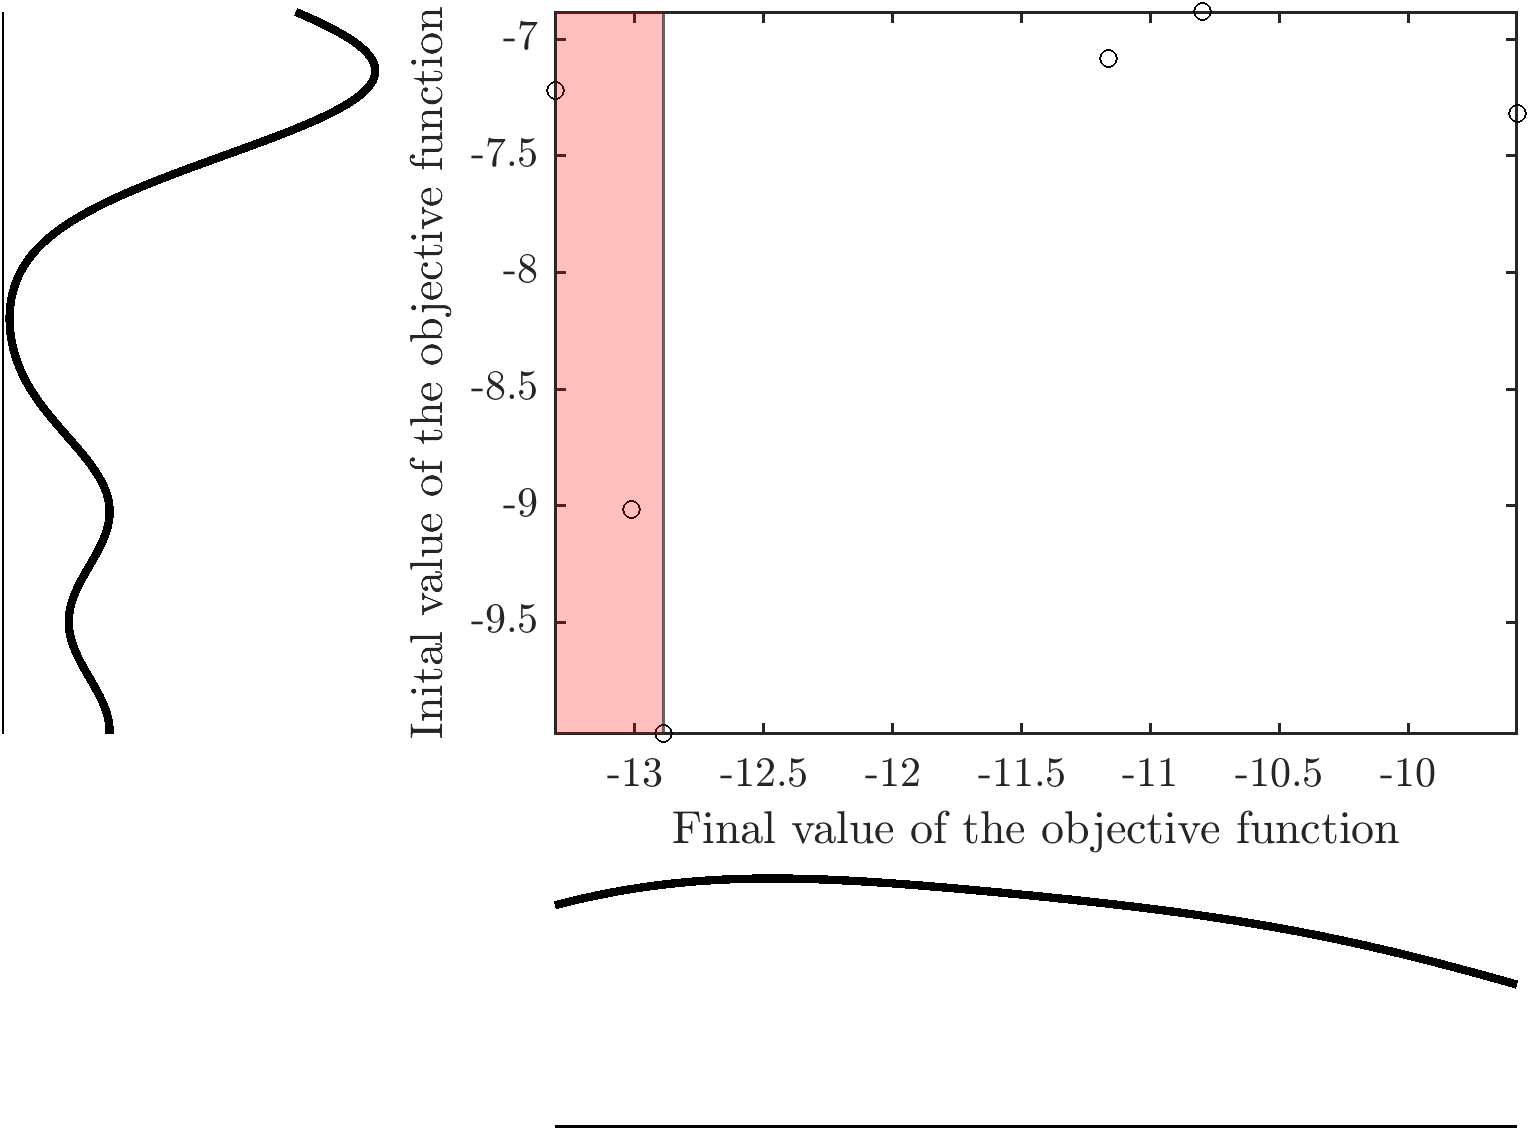
\includegraphics[width=\columnwidth]{Figures/Results/scatter_P.png}	
		\caption{Initial vs final values of the cost function}
		\label{fig:scatter_P}
	\end{figure}
	
	The optimal profiles of pressure and mass flow rate are presented on Figure \ref{fig:profile_P}. Similarly to case 1, only few changes in the mass flow rate are observed in the plot. In contrary to the inlet temperature, the pressure changes are frequently applied in the case 2. 
	
	\begin{figure}[h!]
		\centering
		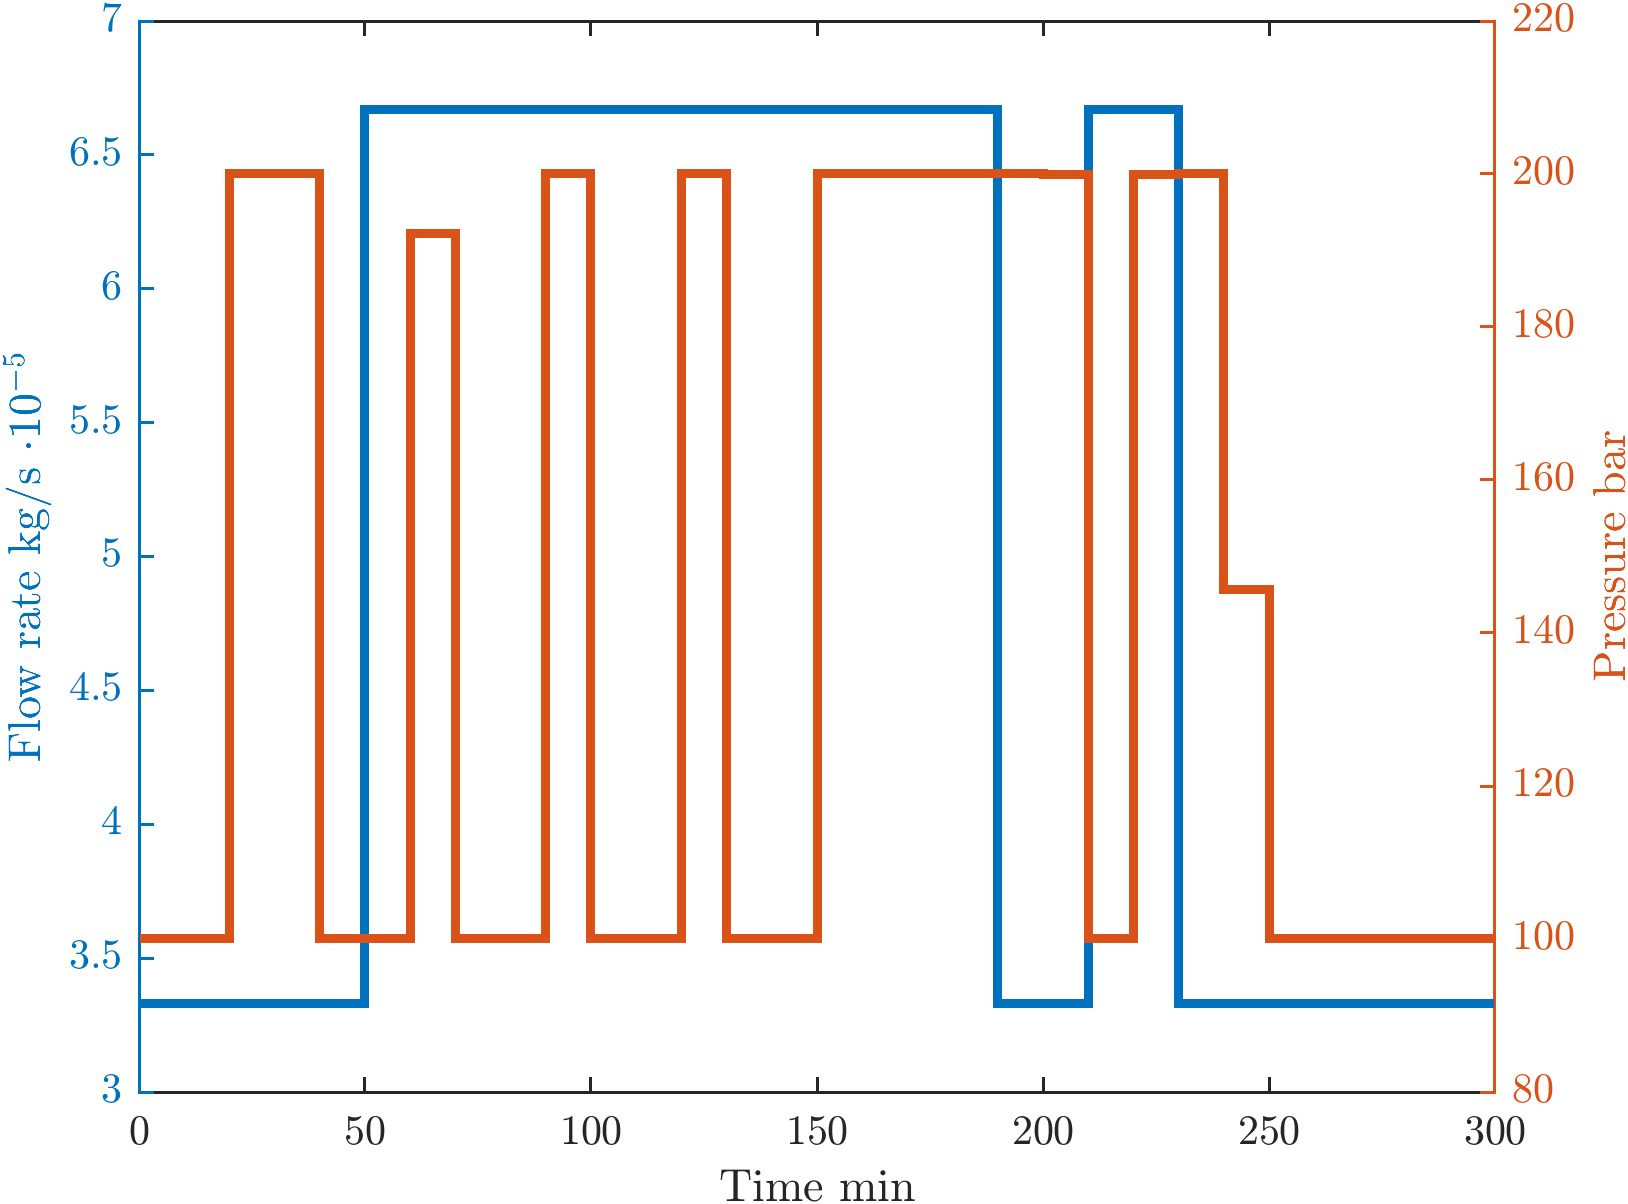
\includegraphics[width=\columnwidth]{Figures/Results/Profile_P_1.png}	
		\caption{Optimal pressure and mass flow rate profiles}
		\label{fig:profile_P}
	\end{figure}
	
	\end{comment}
	
	To identify the global solution of Equations \ref{EQ:Formulation_2},  the optimization problem is solved multiple times, with each run starting from a random initial solution sampled from a uniform distribution. Figure \ref{fig:scatter_T} compares the initial and final values of the cost function across multiple optimization runs for all cases. The solution with the lowest cost function value is considered the global solution for each case.
	
	\begin{figure}[h!]
		\centering
		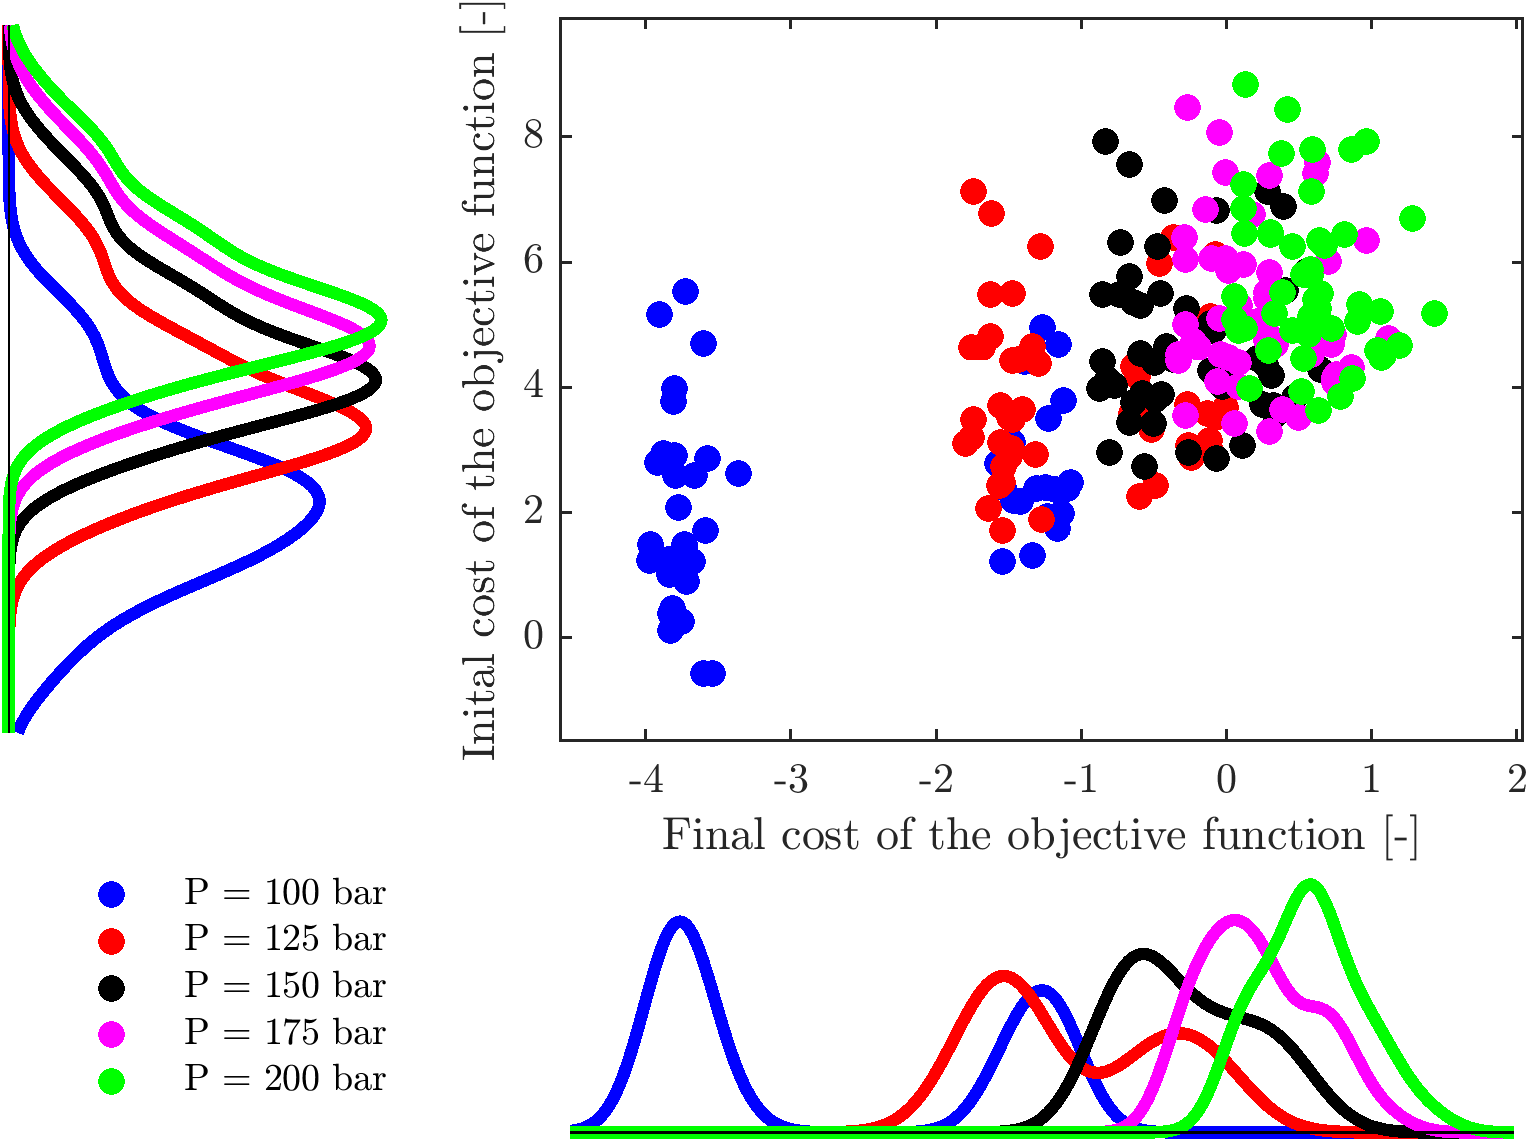
\includegraphics[width=\columnwidth]{Figures/Results/scatter.png}	
		\caption{Initial vs final values of the cost function}
		\label{fig:scatter_T}
	\end{figure}
	
	From Figure \ref{fig:scatter_T}, multiple local solutions are present. The closer the pressure is to the critical point, the greater the deviation in the physical properties of CO$_2$ caused by changes in the inlet temperature, and consequently, the greater the deviation in the Reynolds number, which is one of the independent variables in the analyzed correlation. By examining the clusters visible in Figure \ref{fig:scatter_T}, it can be concluded that experiments conducted at pressures near the supercritical point provide more informative results about the correlation than those performed at pressures farther from it.
	
	\begin{figure}[h!]
		\centering
		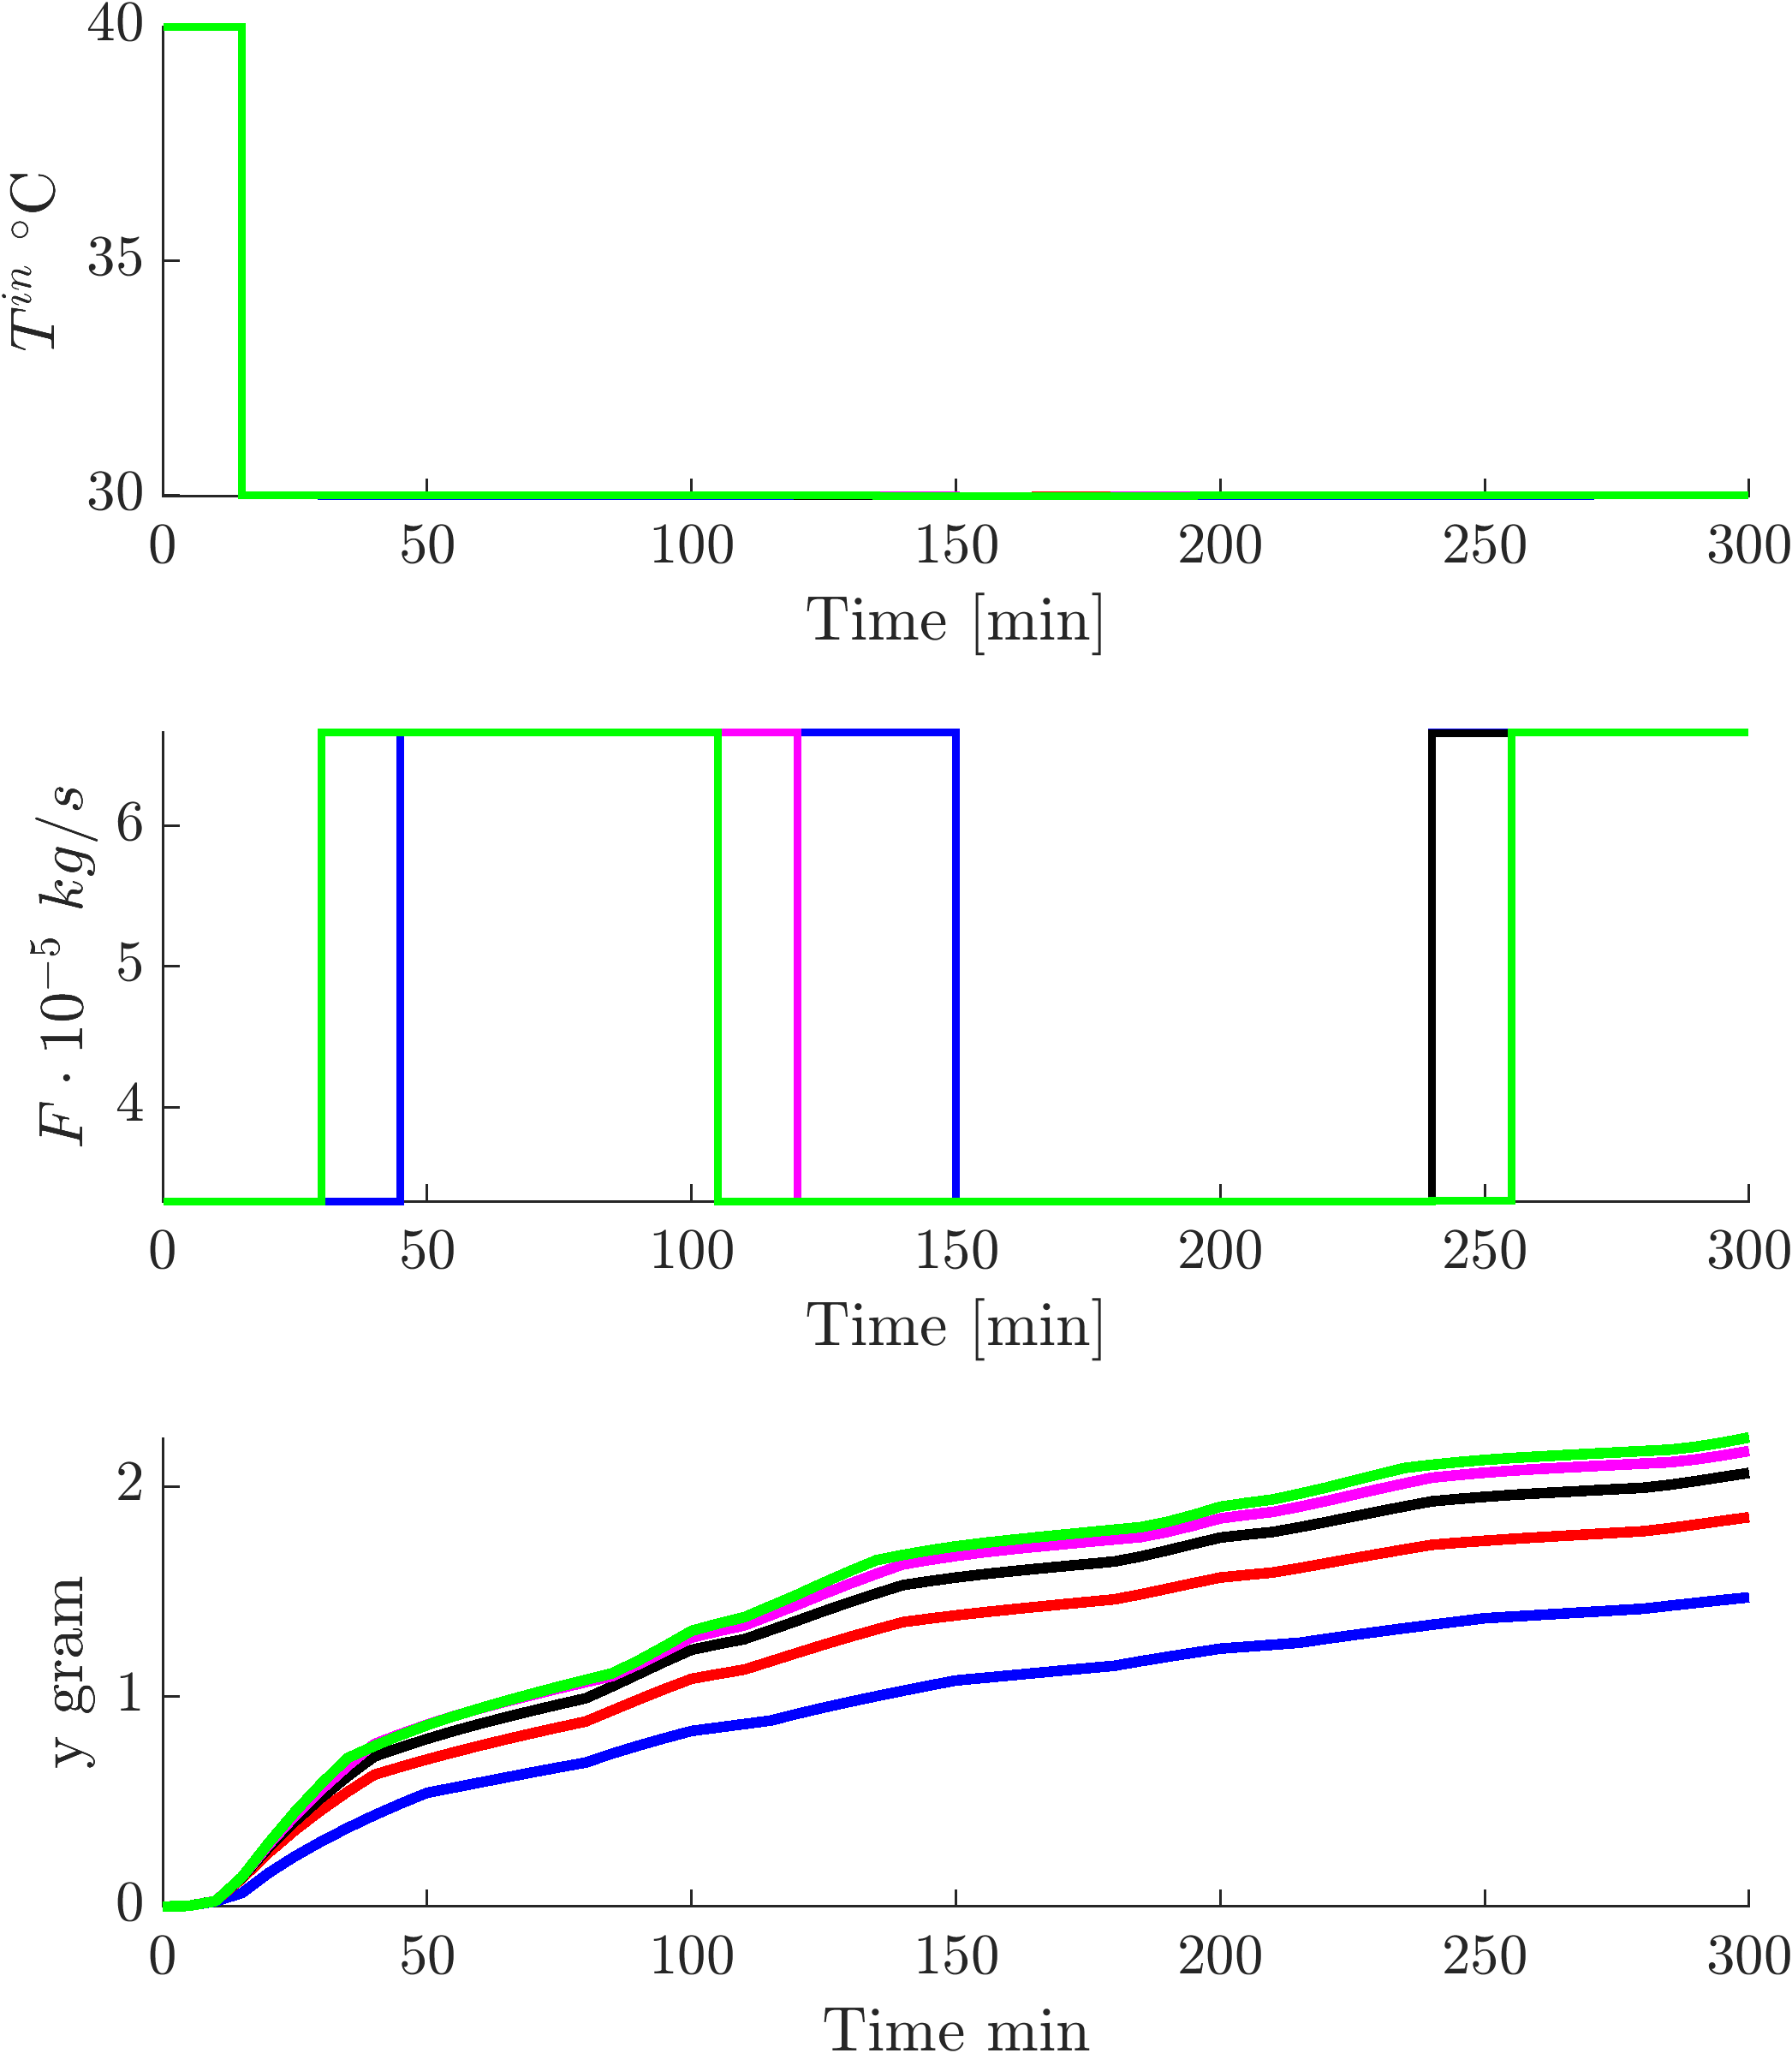
\includegraphics[width=\columnwidth]{Figures/Results/Profiles_all.png}	
		\caption{Optimal profiles}
		\label{fig:profiles}
	\end{figure}
	
\end{document}








































